The Standard Model of Particle Physics (\gls{SM}) \cite{SM} is the description of the physics of elementary particles and their interaction, which is known up to now. The theoretical foundation is the perturbative quantum field theory (\gls{QFT}) which is harmonised with Special Relativity. In the formaslim of \gls{QFT} classical fields are quantized and the information of the interaction of the particles are encoded in the lorentz-invariant lagrangian density $\mathcal{L}$. 



\section{Particles and interactions}
\label{sec:section_1_1}

In the \gls{SM} elementary particles can be characzerized by their spin \cite{SPIN}, which is a quantum number describing an analogon to the intrinsic angular momentum. Fermions carry spin $\frac{1}{2}$ and are represented by Dirac spinors $\psi$, which are complex 4-component objects defined through their behaviour under Lorentz transformation: $\psi^{\alpha}(x) \rightarrow S[\Lambda]^{\alpha}_{\beta} \psi^{\beta}(\Lambda^{-1}x)$ \cite{spinor}. The interaction between the fermions are described by gauge symmetries, which are local symmetry transformations, leaving the langrangian invariant with the introduction of a gauge boson. Gauge boson are elementary particles with spin 1. All relevant symmetries and the corresponding interaction are described in the following, the schematic overview of all elementary particle and their properties are shown in figure \ref{fig:fig_1_1}.

\subsection{U(1)${_e}$ symmetry and quantum electrodynamics (\gls{QED})}
\label{sec:section_1_1_1}

The free langrangian of a fermion, using $\gamma^{\mu}$ as the gamma matrizes and $\bar{\psi} = \psi^{\dagger}\gamma^{0}$, can be written as:

\begin{equation}
	\label{eq:eq_1_1}
	\mathcal{L}_{0} =  i\bar{\psi}(x)\gamma^{\mu}\partial_{\mu}\psi(x) - m\bar{\psi}(x)\psi(x).
\end{equation}

Performing a global transformation of the the kind $\psi(x) \rightarrow \psi'(x) = e^{iQ\alpha}\psi(x)$, with Q and $\alpha$ as real constants, the langrangian stays invariant under this so called U(1) transformation \cite{SM}. The invariance is not fullfilled if $\alpha$ depends explictly on the spacetime $x$, in this case a local gauge transformation is performed. To ensure invariance under a gauge transformation, a new 4-component lorentz vector field $A_{\mu}(x)$ is introduced with following property under U(1) transformation: $A_{\mu} \rightarrow A'_{\mu}(x) = A_{\mu}(x) + \frac{1}{e}\partial_{\mu}\alpha(x)$. Using the definition of the covariant derivate $D_{\mu} = \partial_{\mu} - ieQA_{\mu}(x)$, the following langrangian stays invariant under local U(1) transformation:

\begin{equation}
	\label{eq:eq_1_2}
	\mathcal{L} = i\bar{\psi}(x)\gamma^{\mu}D_{\mu}\psi(x) - m\bar{\psi}(x)\psi(x) = \mathcal{L}_{0} + eQA_{\mu}(x)\bar{\psi}(x)\gamma^{\mu}\psi(x)
\end{equation}

With the gauge transformation the gauge boson of the electromagnetic interaction is introduced, which couples to the fermions with electric charge e: the photon $\gamma$.


\subsection{SU(3)${_C}$ symmetry and quantum chromodynamics (\gls{QCD})}
\label{sec:section_1_1_2}

Beside the electric charge, the so-called quarks are fermions carrying the one of three possible color charges (denoted with r,b,g). Labeling the quark spinor with color $c$ as $q^{c} = \psi_{q}(c)$ and putting them all into a three vector $q_{f} = (q^{b}, q^{r}, q^{g})$, the free lagrangian of quarks can be written as

\begin{equation}
	\label{eq:eq_1_3}
	\mathcal{L}_{0} = \sum_{f} \bar{q_{f}}(i\gamma^{\mu}\partial_{\mu} - m_{f})q_{f}
\end{equation}

The index $f$ denotes the flavour of the quark is explained below. Like in the \gls{QED} example a local gauge theory exists, which introduces gauge bosons. A transformation of the kind $q_{f} \rightarrow q'_{f} = e^{i\frac{\lambda^{a}}{2}\alpha_{a}(x)} q_{f}$, with $\frac{1}{2} \lambda^{a}$ as non communting 3x3 matrixes and $a \in (1, 2, .., 8)$, is a local SU(3)$_{C}$ transformation \cite{QCD}. To get a lagrangian invariant under this tranformation, 8 new gauge bosons $G^{\mu}_{a}(x)$, so-called gluons, have to be introduced, corresponding to the number of generators $\lambda^{a}$ to represent the SU(3)$_{C}$ algebra. Defining the covariant derivative $D_{\mu} = \partial_{\mu}-ig_{s}\frac{\lambda^{a}}{2}G^{\mu}_{a}(x)$ and demand the gluons to transform using $U = e^{i\frac{\lambda^{a}}{2}\alpha_{a}(x)}$ like $G^{\mu}_{a}(x) \rightarrow G^{\mu}(x)' = UG^{\mu}U^{\dagger} - \frac{i}{g_s}(\partial^{\mu}U)U^{\dagger}$ the invariant lagrangian of \gls{QCD} can be written like 

\begin{equation}
	\label{eq:eq_1_4}
	\mathcal{L} = \sum_{f} \bar{q_{f}}(i\gamma^{\mu}D_{\mu} - m_{f})q_{f}
\end{equation}

\subsection{SU(2)$_{W}$ x U(1)$_{Y}$, the electroweak interaction and Higgs mechanism}
\label{sec:section_1_1_3}

The flavour of fermions is a quantum number describing the particle type. For the quarks six different flavours (up, down, charm, strange, top, bottom) exist, for the color-less leptons/neutrinos fermions the three lepton flavour (electron, muon, tau) exist. Beside the flavour the chirality is a key quantity in the electroweak theory, because not all chirality configuration of the fermions couples to the gauge bosons. We define the spinors of fermions with lefthanded(L) or righthanded(R) chirality with $\psi_{L/R} = \frac{1}{2}(1\mp \gamma^{5})\psi$ and for simplizity looking only at the first generation of quarks/leptons, the spinor of quarks/leptons are defined as $u = \psi_{u}, d = \psi_{d}, e = \psi_{e}, \nu = \psi_{\nu_{e}}$. If the fermions are assembled as $q_{L} = (u_{L}, d_{L}), u_{R}, d_{R}, l_{L} = (e_{L}, \nu_{L}), e_{R}$ and consindering them to be massless, the free langrangian of the electroweak theory is

\begin{equation}
	\label{eq:eq_1_5}
	\mathcal{L}_{0} = i\bar{q}_{L}\gamma^{\mu}\partial_{\mu}q_{L} + i\bar{l}_{L}\gamma^{\mu}\partial_{\mu}l_{L} + \sum_{f \in (e, u, d)} i\bar{f}_{R}\gamma^{\mu}\partial_{\mu}f_{R}.
\end{equation}

The local SU(2)$_{W}$ x U(1)$_{Y}$ gauge transformation \cite{EWK}, which is a tranformation of the kind

\begin{equation}
	\label{eq:eq_1_6}
	\begin{split}
		q_{L} \rightarrow q'_{L} = e^{iQ_{q} \alpha_{Y}(x)} e^{i\frac{\sigma_{j}}{2}\alpha^{j}_{W}(x)}q_{L} \\
		l_{L} \rightarrow l'_{L} = e^{iQ_{l} \alpha_{Y}(x)} e^{i\frac{\sigma_{j}}{2}\alpha^{j}_{W}(x)}l_{L} \\
		f_{R} \rightarrow f'_{R} = e^{iQ_{f} \alpha_{Y}(x)}, \quad f \in (e, u, d)
	\end{split}			
\end{equation}

with $\sigma_{j}, j \in (1,2,3)$ as the Pauli matrices, $Q$ as real constant and $a_{Y}, a^{j}_{W}$ as real function of spacetime, introduces 4 gauge bosons, the three $W^{j}_{\mu}(x)$, origating from SU(2)$_{W}$, and the $B_{\mu}$ from U(1)$_{Y}$. Using $U_{L} = e^{i\frac{\sigma_{j}}{2}\alpha^{j}_{W}(x)}$, demanding the transformation properties $B_{\mu} \rightarrow B'_{\mu} = B_{\mu} + \frac{1}{g'}$, $W'_{\mu} \rightarrow U_{L}\frac{\sigma_{j}}{2}W_{\mu}^{j}U_{L}^{\dagger} - \frac{i}{g}(\partial_{\mu}U_{L})U_{L}^{\dagger}$ and defining the covariante derivate 

\begin{equation}
	\label{eq:eq_1_7}
	\begin{split}
		D^{q}_{\mu} = \partial_{\mu}  - ig\frac{\sigma_{j}}{2}W^{j}_{\mu} - ig'Q_{q}B_{\mu} \\
		D^{l}_{\mu} = \partial_{\mu}  - ig\frac{\sigma_{j}}{2}W^{j}_{\mu} - ig'Q_{l}B_{\mu} \\
		D^{f_R}_{\mu} = \partial_{\mu}  - ig'Q_{f}B_{\mu}, \quad f \in (e, u, d)
	\end{split}
\end{equation}

the gauge invariant lagrangian of the electroweak can be written as 

\begin{equation}
	\label{eq:eq_1_8}
	\mathcal{L} = i\bar{q}_{L}\gamma^{\mu}D_{\mu}^{q}q_{L} + i\bar{l}_{L}\gamma^{\mu}D_{\mu}^{l}l_{L} + \sum_{f \in (e, u, d)} i\bar{f}_{R}\gamma^{\mu}D^{f_R}_{\mu}f_{R}
\end{equation}

The problem from this formulation arises from the fact, that the gauge bosons and fermions are measured to have a mass. \\

To explain this discrepancy the Higgs mechanism \cite{HIGGS} is introduced. Considering a complex scalar field doublet $\Phi(x) = (\phi^{1}(x), \phi^{2}(x))$, which transform under SU(2)$_{W}$ like $\Phi(x) \rightarrow \Phi'(x) = e^{iQ_{\Phi} \alpha_{Y}(x)} e^{i\frac{\sigma_{j}}{2}\alpha^{j}_{W}(x)}\Phi(x)$ the lagrangian can be written as

\begin{equation}
	\label{eq:eq_1_9}
	\mathcal{L}_{H} = (D^{\Phi}_{\mu}\Phi)(D^{\Phi, \mu}\Phi)^{\dagger} - \mu^2\Phi^{\dagger}\Phi + \frac{1}{2}(\Phi^{\dagger}\Phi)^2, \quad \mu^2 > 0
\end{equation}

with the covariant derivate $D^{\Phi}_{\mu} = \partial_{\mu}  - ig\frac{\sigma_{j}}{2}W^{j}_{\mu} - ig'Q_{\Phi}B_{\mu}$. Because of the condition for $\mu$, the vacuum expectation value of $\Phi$ is non vanishing: $\Phi\Phi^{\dagger} = \frac{\mu^2}{\lambda} \equiv \nu$. One of the four degrees of freedom of $\Phi$ is set with this condition, the other free degrees of freedem can be removed by a gauge transformation. Choosing the unitary gauge, $\Phi$ can be written as $\Phi = (\nu + \frac{1}{\sqrt{2}}H(x), 0)$, with $H(x)$ as the scalar spin 0 field, called Higgs boson. Plugging this into equation \ref{eq:eq_1_9}, the following show up

\begin{equation}
	\label{eq:eq_1_10}
	\begin{split}
		Z_{\mu} = \cos(\theta_{W})W^{3}_{\mu} + \sin(\theta_{W})B_{\mu}, \quad M_{Z} = \frac{1}{2}(g^2 + g'^2)\nu^2 \\
		A_{\mu} = -\sin(\theta_{W})W^{3}_{\mu} + \sin(\theta_{W})B_{\mu}, \quad M_{A} = 0 \\
		W^{\pm}_{\mu} = \frac{1}{\sqrt{2}}W^{1}_{\mu} \mp W^{2}_{\mu}, \quad M_{W} = \frac{1}2{\sqrt{2}}(g^2+g'^2)\nu^2
	\end{split}
\end{equation}

The $Z$ boson and the $W^{\pm}$ from the weak interaction appeared with the introduction of the Higgs \cite{HIGGDISCOVER}, which are both massiv, like measured in nature. Also the photon $A_{\mu}$, which also come up during the \gls{QED} discussion, appeared with zero mass. 


\begin{figure}[hpt]
	\centering
	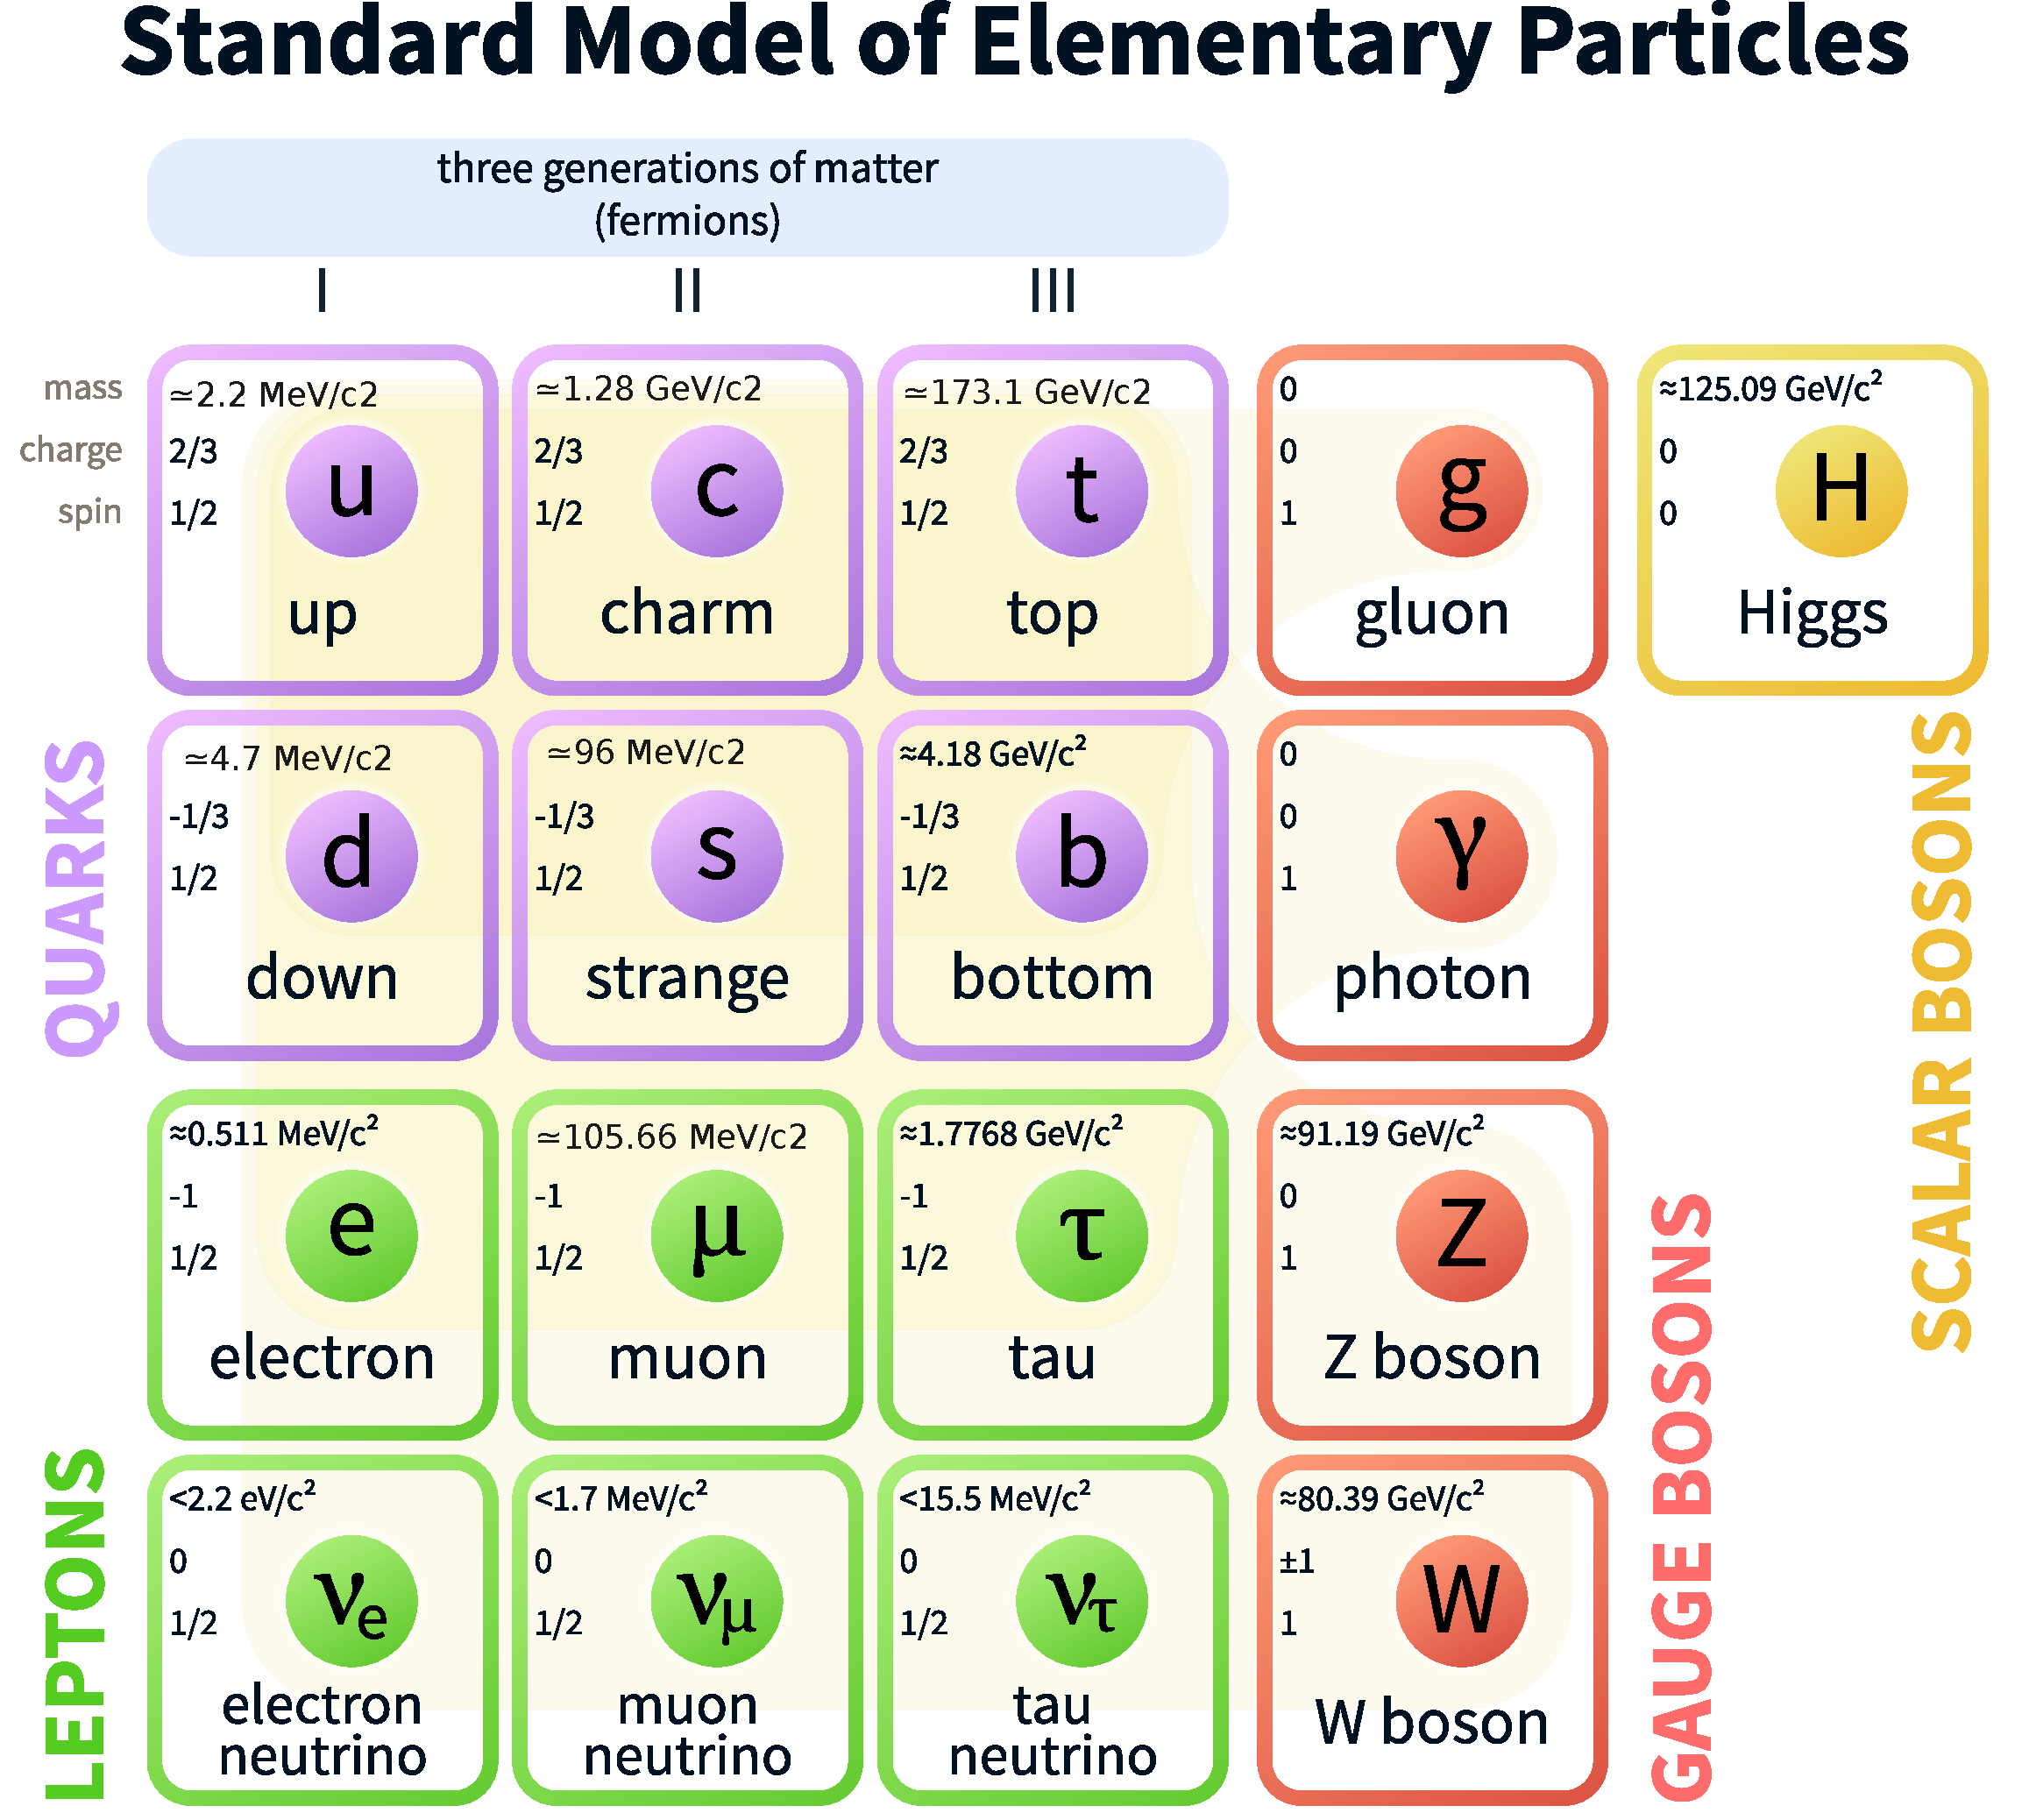
\includegraphics[width=0.8\textwidth]{pictures/Standard_Model_of_Elementary_Particles.pdf}

	\caption[Schematic overwiev of Standard Model particles]{Schematic overview of all known elementary particles of the \gls{SM} with their measured properties, taken from \cite{SMPARTICLES}}
	\label{fig:fig_1_1}
\end{figure}

\section{Symmetries and conservation}
\label{sec:section_1_2}

Symmetries in a physical system and conservation laws are directly coupled, not only in \gls{QFT}. The central theoretical foundation is the Noether theorem \cite{NOTHERTHEOREM}. It states that a symmetry in the physical system leads to a conservation law. In terms of \gls{QFT} the Noether theorem says that if a field $\phi(x)$ exists, which langrangian $\mathcal{L}$ is invariant under the infinitesimal transformation $\phi(x) \rightarrow \phi'(x) = \phi(x) + \alpha \delta \phi(x)$, then a current $j^{\mu}$ exists, which is conversed: $\partial_{\mu}j^{\mu} = 0$.  

\subsection{Example of conservation in \gls{QED}}
\label{sec:section_1_2_1}

In section \ref{sec:section_1_1_1} the U(1) symmetry in \gls{QED} is discussed. Without loss of generality looking at a global U(1) transformation, which means $\alpha$ is a real constant, the infinitesimal transformation of the spinor is done by $\psi(x) \rightarrow \psi'(x) = \psi(x) + \alpha \delta \psi(x)$ and  $\bar{\psi}(x) \rightarrow \bar{\psi}'(x) = \bar{\psi}(x) - \alpha \delta \bar{\psi}(x)$. The free langrangian in equation \ref{eq:eq_1_1} is invariant under this tranformation, so it exist a conserved current $j_{\text{QED}}^{\mu}$. Defining the charge $Q_{\text{QED}} = \int j^{0}_{\text{QED}} d^{3}x$, equation \ref{eq:eq_1_11} shows a conserved charge. 

\begin{equation}
	\label{eq:eq_1_11}
	\frac{d}{dt} Q_{\text{QED}} = \int \frac{d}{dt}j^{0}_{\text{QED}}d^{3}x \overset{\partial_{\mu}j_{\text{QED}}^{\mu} = 0}{=} \int \vec{\nabla} \vec{j}_{\text{QED}}d^{3}x \overset{\text{Boundary conditions}}{=} 0
\end{equation}

In the example of the \gls{QED} the conserved charge is the electric charge of the fermion.

\subsection{Conversation laws in the \gls{SM}}
\label{sec:section_1_2_2}

In the \gls{SM} different type of symmetries give rise to conversation laws. The first type are the gauge symmetries, which lead to the consevation of the charge of the corresponding interaction. The second type are continous Lorentz transformation, including translation/rotation symmetries, and the third type are discrete transformations, including space/time inversion and charge conjugation \cite{Peskin}. All conservation quantities and the corresponding symmetry are listed in table \ref{tab:tab_1_1}.

\begin{table}[h]
	\centering
	\caption[Symmetries in the Standard Model]{Symmetries and the corresponding conserved quantities in the \gls{SM}. The second column shows the transformation property of a generic quantum field $\phi(x)$, which langrangian have to stay invariant to fullfill Noethers theorem}
	\label{tab:tab_1_1}

	\begin{tabular}{l|l|l}
		Symmetry					&Transformation										&Conserved quantity			\\ \hline
			
		SU(2)$_{W}$ x U(1)$_{Y}$			&see equation \ref{eq:eq_1_6}								&$Y = 2(Q - I_{3})$ (hyper charge)	\\ \hline
		
		SU(3)$_{C}$					&$q_{f} \rightarrow q'_{f} = e^{i\frac{\lambda^{a}}{2}\alpha_{a}(x)} q_{f}$		&Colour charge				\\ \hline \hline

		Space time translation 				&$\phi(x) \rightarrow \phi'(x) = \phi(x + a)$						&Energy/Momentum			\\ \hline

		Rotation					&$\phi(x) \rightarrow \phi'(x) = \phi(Rx)$						&Angular momentum			\\ \hline \hline

		Space inversion					&$\phi(\vec{x}, t) \rightarrow \phi'(\vec{x}, t) = \phi(-\vec{x}, t)$			&Parity					\\ \hline
		
		Time inversion					&$\phi(\vec{x}, t) \rightarrow \phi'(\vec{x}, t) = \phi(\vec{x}, -t)$	 		&Entropy				\\ \hline

		Charge conjugation				&$\phi(x) \rightarrow \phi'(x) = \phi(x)^{\dagger}$					&C-parity				
	\end{tabular}
\end{table}



\section{Lepton flavour violation}
\label{sec:section_1_3}

In the \gls{SM} two types of quantum numbers are assigned to leptonic fermions. The lepton number $L$ assigns the value 1/-1 to all leptonic fermions/anti fermions, and zero to everything else. Im comparison to that the lepton flavour $L_{\ell}$ with $\ell \in (e, \mu, \tau)$ assigns 1/-1 to the lepton/anti lepton with flavour $\ell$, zero to everything else. A overwiew is shown in table \ref{tab:tab_1_2}


\begin{table}[h]
	\centering
	\caption[Lepton number/lepton flavour of leptons]{Lepton number/lepton flavour for all known leptons in the \gls{SM}}
	\label{tab:tab_1_2}

	\begin{tabular}{l|l|l|l|l}
		Lepton				&$L$		&$L_{e}$	&$L_{\mu}$	&$L_{\tau}$	\\ \hline
		
		$e^{-}/e^{+}$			&$\pm 1$	&$\pm 1$	&0		&0		\\

		$v_{e}/\bar{v}_{e}$		&$\pm 1$	&$\pm 1$	&0		&0		\\
		
		$\mu^{-}/\mu^{+}$		&$\pm 1$	&0		&$\pm 1$	&0		\\

		$v_{\mu}/\bar{v}_{\mu}$		&$\pm 1$	&0		&$\pm 1$	&0		\\
		
		$\tau^{-}/\tau^{+}$		&$\pm 1$	&0		&0		&$\pm 1$	\\

		$v_{\tau}/\bar{v}_{\tau}$	&$\pm 1$	&0		&0		&$\pm 1$	\\			
	\end{tabular}
\end{table}


\subsection{Global lepton flavour symmetry}
\label{sec:section_1_3_1}

The \gls{SM} Langragian $\mathcal{L}^{\ell}_{\text{SM}}$ \cite{Peskin, EWK}, only looking at the parts where leptons are involved, and after introducing the Higgs bosons, like discussed in section \ref{sec:section_1_1}, can be written as

\begin{multline}
	\label{eq:eq_1_12}
	\mathcal{L}^{\ell}_{\text{SM}} = \sum_{f \in (e, \mu, \tau)} \underbrace{-(1+\frac{H}{\nu}) m_{f} \bar{f}f}_\text{Higgs coupling} + \underbrace{\frac{g}{\sqrt{2}} (W^{+}_{\mu} \bar{\nu}^{f}_{L} \gamma^{\mu} f_{L} + W^{-}_{\mu} \bar{f}_{L} \gamma^{\mu} \nu^{f}_{L})}_{W^{\pm} \text{ coupling}} \\
	+ \underbrace{\frac{g}{\cos{\theta_{W}}}(Z_{\mu} \frac{1}{2} \bar{\nu}^{f}_{L} \gamma^{\mu}\nu^{f}_{L} + \bar{f}_{L}(-\frac{1}{2} + \sin^2{\theta_{W}})f_{L} + \bar{f}_{R}(\sin^2{\theta_{W}})f_{L}}_{\text{Z coupling}} - \underbrace{eA_{\mu}\bar{f}\gamma^{\mu}f}_{\text{photon coupling}}.
\end{multline}

This langrangian is invariant under global flavour transformation U(1)$_{e}$ x U(1)$_{\mu}$ x U(1)$_{\tau}$ \cite{LFV1, LFV2}, which is a transformation of kind 

\begin{equation}
	\label{eq:eq_1_13}
	\begin{split}
		f \rightarrow f' = e^{i\alpha_{\ell}Q_{f}}f, \quad f \in (e, \mu, \tau) \\
		\nu^{f} \rightarrow \nu'^{f} = e^{i\alpha_{f}Q_{f}}\nu^{f}, \quad f \in (e, \mu, \tau) \\
	\end{split}
\end{equation}

with $Q_{f}$ and $\alpha_{\ell}$ as real constants. In comparison to the gauge symmetries this symmetry introcudes no new gauge boson, a $\alpha_{\ell}$ dependence of $x$ would spoil the symmetry and cannot be fixed by a gauge boson introduction. The flavour symmetry, due to the Noether theorem, introduces conserved quantities, which are the lepton flavour introduced in the beginning of section \ref{sec:section_1_3}.


\subsection{Breaking of the symmetry due to neutrino masses}
\label{sec:section_1_3_2}

The Langrangian in equation \ref{eq:eq_1_12} does not include mass terms for neutrinos, because to non observed $\nu_R$, which leads to a vanishing neutrino mass term $-m_{\nu^{f}}\bar{\nu}^{f}\nu^{f} = -m_{\nu^{f}_{L}}\bar{\nu}^{f}_{R}\nu^{f}_{L} + {\nu}^{f}_{L}\bar{\nu}^{f}_{R} = 0$. But in difference to the \gls{SM} prediction, neutrinos have a non-vanshing mass, due to the measurement of neutrino oscillation \cite{NEUTRINOOSC}. This phenomena describe change of lepton flavour of the neutrinos, which is possible because flavour eigenstates are not equal to the mass eigenstates $|\nu_{f}> \neq |\nu_{m_{f}}>$ and are connected via the unitary 3x3 PMNS matrix $U$ \cite{PMNS}: $|\nu_{f}> =  \sum_{i} U^{i}_{f}|\nu_{m_{i}}>$. The probability P of the transitation from flavour $\alpha$ to flavour $\beta$ \cite{NEUTRINOPROB} is given by 

\begin{equation}
	\label{eq:eq_1_14}
	P(\alpha \rightarrow \beta) = |\sum_{i, j} U_{\alpha}^{i} U_{\beta}^{j} e^{i\Delta m^2_{ij}L/(2E)}|^2
\end{equation}

There are two possible ways to introduce neutrino mass terms in an extended \gls{SM} langrangian. With the introduction of right handed neutrinos (dirac type) or postulating what left-handed neutrinos are particle/anti-particle at the same time (majorana type), the most general langrangians including neutrino mass terms \cite{NEUTRINOMASS} can be written as 

\begin{equation}
	\label{eq:eq_1_15}
	\begin{split}
		\mathcal{L}_{\text{Dirac}} = -\bar{\nu}^{\ell'}_{R}M^{\text{Dirac}}_{\ell'\ell} \nu^{\ell}_{L} + \text{h.c.} \\
		\mathcal{L}_{\text{Majorana}} = -C(\bar{\nu}^{\ell'}_{L})^{T}M^{\text{Majorana}}_{\ell'\ell} \nu^{\ell}_{L} + \text{h.c.} 
	\end{split}
\end{equation}

with $M_{\ell'\ell}$ as complex 3x3 matrix, which is not diagonal, because of the different mass/flavour eigenstates of neutrinos. This leads to the breaking of the flavour symmetry, because $\mathcal{L}_{\text{Dirac}}$/$\mathcal{L}_{\text{Majorana}}$ are not invariant under the flavour transformation in equation \ref{eq:eq_1_13}. Neutrino masses introduces lepton flavour violation (\gls{LFV}), and branching ratios on neutrino mixing induced \gls{LFV} Z boson decays \cite{NEUTRINOLFV} can be calculated to be 

\begin{equation}
	\label{eq:eq_1_16}
	\begin{split}
		\text{BR}^{\nu \text{ mix}}(Z\to e\mu) < 10^{-55} \\
		\text{BR}^{\nu \text{ mix}}(Z\to e\tau) < 10^{-54} \\
		\text{BR}^{\nu \text{ mix}}(Z\to \mu\tau) < 10^{-60}
	\end{split}
\end{equation}

This branchings ratios are far away from being detectable, which leads to a good approximation of conservation of lepton flavour, even with massive neutrinos.

\subsection{Lepton flavour violation beyond the Standard model}
\label{sec:section_1_3_3}

The discussion in section \ref{sec:section_1_3_2} showed, that lepton flavour symmetry is not absolute and can be broken. In the case of neutrino mixing induced \gls{LFV} non observable rates are predicted. But if \gls{LFV} would be found on a measurable level, it would imply that another process in a beyond the Standard Model (\gls{BSM}) theory exists, which breaks lepton flavour symmetry. So \gls{LFV} can be used as a probe and a getway to \gls{BSM} theories. \\

One example of such a theory is the specific supersymmetric extension of the standard model \cite{SUSYLFV}, which could predict \gls{BSM} \gls{LFV} decays. But a more convenient way to probe \gls{BSM} is to search in a model-independent approach, because a specific \gls{LFV} model is not nessecarily realized, but \gls{LFV} could still exist because of another realisation in nature. So to search for example a \gls{LFV} Z decay without any underlying model give rise to the possibility to find \gls{BSM} physics, without constraints due to the specific model dependent phase space. \\

Previous searches for \gls{LFV} in Z bosons were performed and giving first contraints on the branching ratios. In the $e\mu$ final state the best result is published by Compact Muon Solenoid (\gls{CMS}) using data from RunI at $\sqrt{s} = 8$ TeV and given by the limit of the branching ratios $\text{BR}(Z\to e\mu) < 7.3\cdot 10^{-7}$ \cite{LFVEMU}. The limits in the $e\tau$ and $\mu\tau$ final state are measured at the Large Electron-Positron Collider (\gls{LEP}) \cite{LEP} collider using data from the run in the years 1991-1993 and are given by the result from the OPAL detector $\text{BR}(Z\to e\tau) < 9.8\cdot 10^{-6}$ \cite{LFVETAU} and from the DELPHI detector $\text{BR}(Z\to \mu\tau) < 1.2\cdot 10^{-5}$ \cite{LFVMUTAU}.
